\begin{frame}{Learning Rate}
    \begin{itemize}
        \item Learning rate is a hyper-parameter that controls how much we are adjusting the weights of our network with respect the loss gradient. 
        \begin{figure}[H]
    		\centering
    		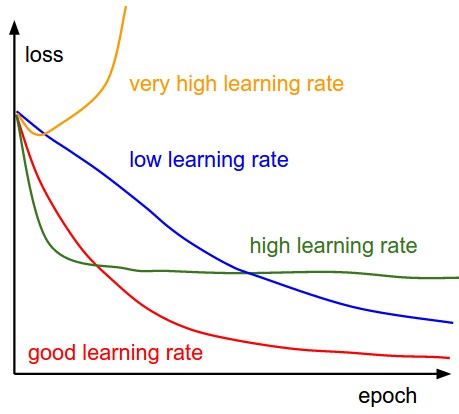
\includegraphics[width=0.5\textwidth]{Figs/lr.png}
    		\caption{Learning Rate Effect}
	    \end{figure}
    \end{itemize}        
\end{frame}

\begin{frame}{Learning Rate}
    \begin{itemize}
	    \item While this might be a good idea (using a low learning rate) in terms of making sure that we do not miss any local minima, it could also mean that we’ll be taking a long time to converge
    \end{itemize}  
    \begin{figure}[H]
    		\centering
    		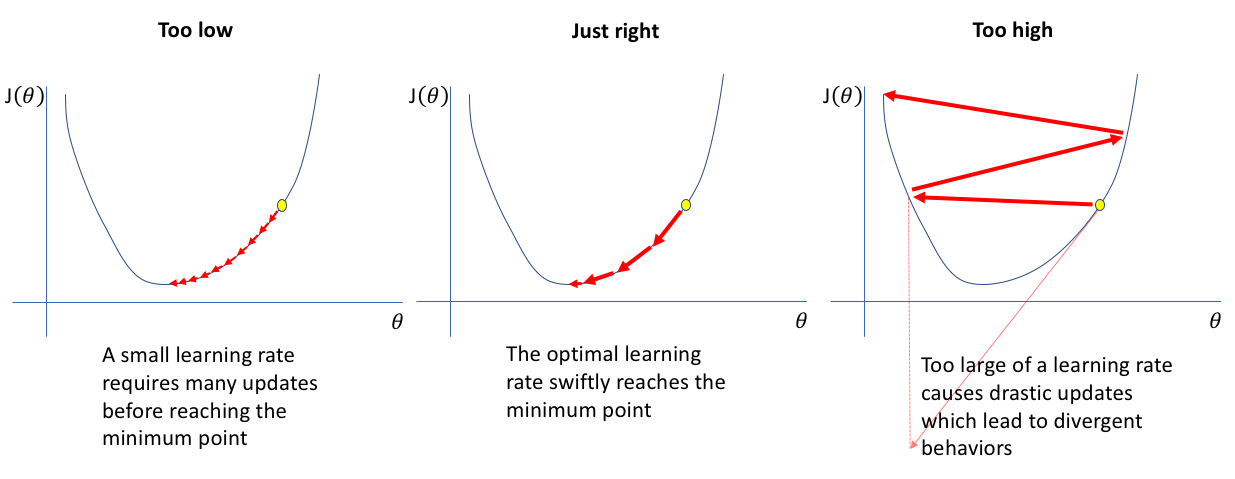
\includegraphics[width=0.7\textwidth]{Figs/lr_2.png}
    		\caption{Learning Rate Effect}
    \end{figure}
\end{frame}

\begin{frame}{Learning Rate}
	    \begin{figure}[H]
    		\centering
    		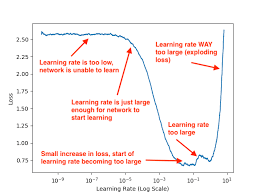
\includegraphics[width=0.7\textwidth]{Figs/lr_5.png}
    		\caption{Learning Rate Effect}
	    \end{figure}
\end{frame}

\begin{frame}{Vanishing/Exploding Gradient}
    \begin{figure}[H]
    		\centering
    		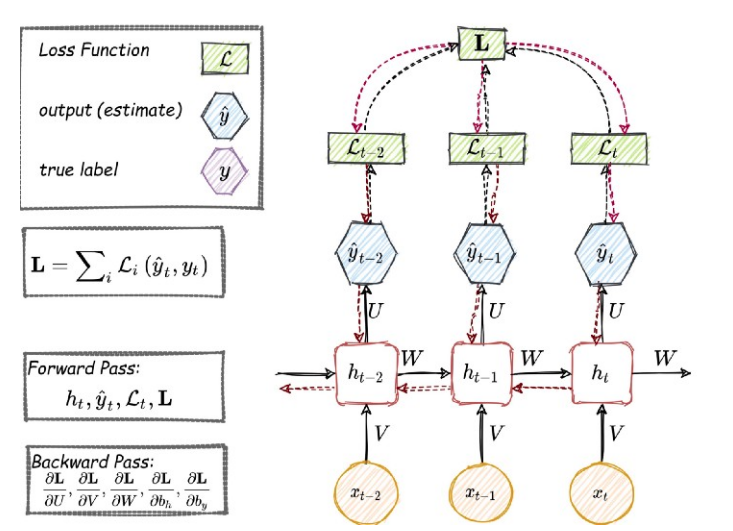
\includegraphics[width=0.7\textwidth]{Figs/van3.png}
    		\caption{Vanishing/Explode}
	    \end{figure}
\end{frame}

\begin{frame}{Vanishing/Exploding Gradient}
    \begin{figure}[H]
    		\centering
    		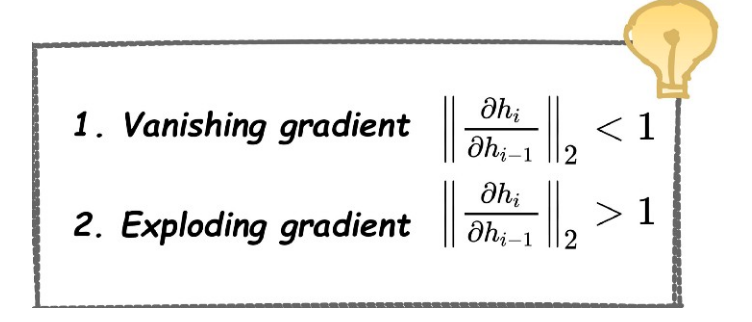
\includegraphics[width=0.7\textwidth]{Figs/van4.png}
    		\caption{Vanishing/Explode}
	    \end{figure}
\end{frame}

\begin{frame}{Vanishing/Exploding Gradient Cont.}
    \begin{itemize}
        \item Exploding
        \begin{itemize}
            \item Causes the gradient descent to diverge. 
        \end{itemize}
        \item Vanishing
        \begin{itemize}
            \item Gradient descent never converges to the optimum. 
        \end{itemize}
    \end{itemize}
    \begin{figure}[H]
    		\centering
    		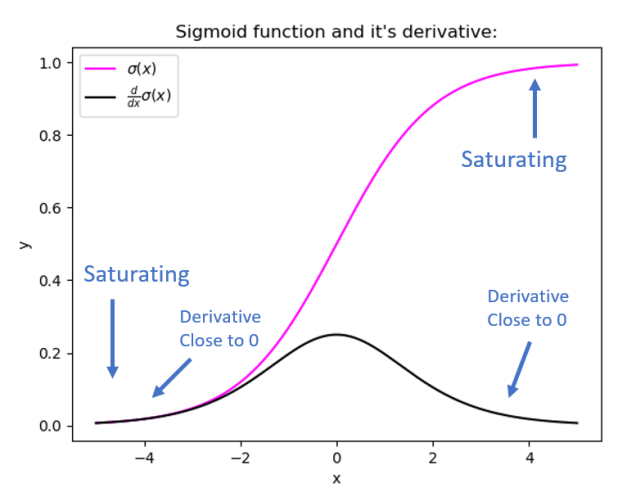
\includegraphics[width=0.5\textwidth]{Figs/van_1.png}
    		\caption{Vanishing/Explode Derivatives}
	    \end{figure}
\end{frame}

\begin{frame}{Vanishing/Exploding Gradient Cont.}
    \begin{itemize}
        \item Exploding
        \begin{itemize}
            \item The model is not learning much on the training data therefore resulting in a poor loss.
        \end{itemize}
        \item Vanishing
        \begin{itemize}
            \item Model weights shrink exponentially and become very small when training the model.
        \end{itemize}
    \end{itemize}
\end{frame}

\begin{frame}{Vanishing/Exploding Gradient Cont.}
    \begin{itemize}
        \item How to Prevent? 
        \begin{itemize}
            \item The variance of outputs of each layer should be equal to the variance of its inputs.
            \item The gradients should have equal variance before and after flowing through a layer in the reverse direction.
        \end{itemize}
    \end{itemize}
\end{frame}

\DeclarePairedDelimiter\abs{\lvert}{\rvert}%
\begin{frame}{Saturating Functions}
    \begin{itemize}
        \item Intuition
        \begin{itemize}
            \item A saturating activation function squeezes the input.
        \end{itemize}
        \item Definition
        \begin{align*}
            (\abs{\lim_{z\hookrightarrow -\infty}f(z)=+\infty})
            \vee (\abs{\lim_{z\hookrightarrow +\infty}f(z)=+\infty})
        \end{align*}
        
    \end{itemize}
\end{frame}

\begin{frame}{Saturating Functions Cont.}
    \begin{itemize}
            \item The tanh (hyperbolic tangent) activation function is saturating as it squashes real numbers to range between $(-1, 1)$
            \begin{figure}[H]
    		     \centering
    		     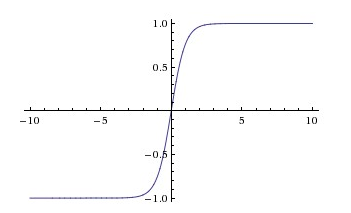
\includegraphics[width=0.5\textwidth]{Figs/tanh.png}
    		     \caption{Tanh}
	        \end{figure}
    \end{itemize}
\end{frame}

\begin{frame}{Saturating Functions Cont.}
    \begin{itemize}
            \item The sigmoid activation function  $f(x) = \frac{1}{1+\exp^{-x}}$ is also saturating, because it squashes real numbers to range between $(0, 1)$.
            \begin{figure}[H]
    		     \centering
    		     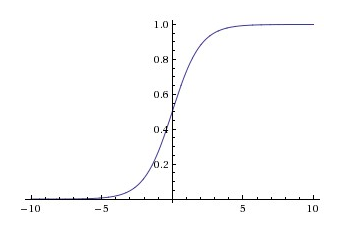
\includegraphics[width=0.5\textwidth]{Figs/sig.png}
    		     \caption{Sigmoid}
	        \end{figure}            
    \end{itemize}
\end{frame}

\begin{frame}{Saturating Functions Cont.}
    \begin{itemize}
            \item In contrast, The Rectified Linear Unit (ReLU) activation function is non-saturating.
            \begin{figure}[H]
    		     \centering
    		     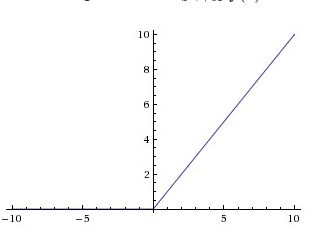
\includegraphics[width=0.5\textwidth]{Figs/relu.png}
    		     \caption{Relu}
	        \end{figure}             
    \end{itemize}
\end{frame}
